\documentclass[12pt]{article}
\usepackage[margin=0.75in]{geometry}
\usepackage{float}
\usepackage{multicol}
\usepackage{lmodern}
\usepackage{amssymb,amsmath}
\usepackage{ifxetex,ifluatex}
\usepackage{fixltx2e} % provides \textsubscript
\ifnum 0\ifxetex 1\fi\ifluatex 1\fi=0 % if pdftex
  \usepackage[T1]{fontenc}
  \usepackage[utf8]{inputenc}
\else % if luatex or xelatex
  \ifxetex
    \usepackage{mathspec}
    \usepackage{xltxtra,xunicode}
  \else
    \usepackage{fontspec}
  \fi
  \defaultfontfeatures{Mapping=tex-text,Scale=MatchLowercase}
  \newcommand{\euro}{€}
\fi
% use upquote if available, for straight quotes in verbatim environments
\IfFileExists{upquote.sty}{\usepackage{upquote}}{}
% use microtype if available
\IfFileExists{microtype.sty}{%
\usepackage{microtype}
\UseMicrotypeSet[protrusion]{basicmath} % disable protrusion for tt fonts
}{}
\usepackage{longtable,booktabs}
\usepackage{graphicx}
\makeatletter
\def\maxwidth{\ifdim\Gin@nat@width>\linewidth\linewidth\else\Gin@nat@width\fi}
\def\maxheight{\ifdim\Gin@nat@height>\textheight\textheight\else\Gin@nat@height\fi}
\makeatother
% Scale images if necessary, so that they will not overflow the page
% margins by default, and it is still possible to overwrite the defaults
% using explicit options in \includegraphics[width=3.5in][width, height, ...]{}
\setkeys{Gin}{width=\maxwidth,height=\maxheight,keepaspectratio}
\ifxetex
  \usepackage[setpagesize=false, % page size defined by xetex
              unicode=false, % unicode breaks when used with xetex
              xetex]{hyperref}
\else
  \usepackage[unicode=true]{hyperref}
\fi
\hypersetup{breaklinks=true,
            bookmarks=true,
            pdfauthor={Brandon LeBeau},
            pdftitle={PSQF 4143: Section 11},
            colorlinks=true,
            citecolor=blue,
            urlcolor=blue,
            linkcolor=magenta,
            pdfborder={0 0 0}}
\urlstyle{same}  % don't use monospace font for urls
\setlength{\parindent}{0pt}
\setlength{\parskip}{6pt plus 2pt minus 1pt}
\setlength{\emergencystretch}{3em}  % prevent overfull lines
\setcounter{secnumdepth}{0}

\title{PSQF 4143: Section 11}
\author{Brandon LeBeau}
\date{}

\begin{document}
\maketitle

\section{Possible Errors}\label{possible-errors}

\begin{itemize}
\itemsep1pt\parskip0pt\parsep0pt
\item
  In making a conclusion from our statistical analysis, there are four
  possible conclusions that can be made:

  \begin{enumerate}
  \def\labelenumi{\arabic{enumi}.}
  \itemsep1pt\parskip0pt\parsep0pt
  \item
    Reject the null hypothesis that is false (correct conclusion).
  \item
    Fail to reject a null hypothesis that is true (correct conclusion).
  \item
    Reject a null hypothesis even though it is true (Type I Error).
  \item
    Fail to reject a null hypothesis even though it is false (Type II
    Error).
  \end{enumerate}
\end{itemize}

\section{Type I and Type II Errors}\label{type-i-and-type-ii-errors}

\begin{longtable}[c]{@{}lll@{}}
\toprule
\textasciitilde{} & \(H_{0}\) is true & \(H_{0}\) is
false\tabularnewline
\midrule
\endhead
Reject \(H_{0}\) & Type I Error \(\alpha\) & Correct
\(1 - \beta\)\tabularnewline
Fail to reject \$H\_\{0\} & Correct \(1-\alpha\) & Type II Error
\(\beta\)\tabularnewline
\bottomrule
\end{longtable}

\section{Type I Errors}\label{type-i-errors}

\begin{itemize}
\itemsep1pt\parskip0pt\parsep0pt
\item
  Type I Error occurs when we find an effect or relationship in our
  sample that is not in the population.

  \begin{itemize}
  \itemsep1pt\parskip0pt\parsep0pt
  \item
    Have a significant result when in fact it is not significant.
  \item
    Reject a true null hypothesis.
  \item
    The probability of a Type I Error \(= \alpha\).
  \item
    The conventional (historical) \(\alpha\) value is .05.
  \item
    Since the probability of a Type I Error is \(\alpha\), the
    researcher has direct control over how likely a Type I Error would
    occur.
  \item
    Using an \(\alpha = .05\) means that even when no difference exists
    in the population, 5\% of random samples will show a significant
    difference.
  \item
    To reduct type I errors, simply use a smaller \(\alpha\), (i.e. .01
    or .001).
  \end{itemize}
\end{itemize}

\section{Type II Errors}\label{type-ii-errors}

\begin{itemize}
\itemsep1pt\parskip0pt\parsep0pt
\item
  Type II Error occurs when we do not find an effect or relationship in
  our sample that exists in the population.

  \begin{itemize}
  \itemsep1pt\parskip0pt\parsep0pt
  \item
    Have a non-significant result when in fact it is significant.
  \item
    Fail to reject a false null hypothesis.
  \item
    Probability of a Type II Error \(= \beta\)
  \end{itemize}
\item
  Type II Errors (\(\beta\)) depends on the size of the difference in
  the population and the sample size.
\item
  A similar measure is \textbf{power} (\(1-\beta\)), the probability
  that a study will produce a statistically significant result
  \textbf{if the research hypothesis is true}.
\item
  The conventional level for power is .8, this is what researchers
  strive for when planning a research study.
\end{itemize}

\section{Type I and Type II Error
Example}\label{type-i-and-type-ii-error-example}

\begin{itemize}
\itemsep1pt\parskip0pt\parsep0pt
\item
  Suppose we're interested in examining the safety of a drug.

  \begin{itemize}
  \itemsep1pt\parskip0pt\parsep0pt
  \item
    \(H_{0}\): The drug is unsafe.
  \item
    \(H_{1}\): The drug is safe.
  \end{itemize}
\item
  What is the type I error?

  \begin{itemize}
  \itemsep1pt\parskip0pt\parsep0pt
  \item
    Reject \(H_{0}\) when true; more specifically, conclude drug is safe
    when in fact it is unsafe.
  \end{itemize}
\item
  What is the type II error?

  \begin{itemize}
  \itemsep1pt\parskip0pt\parsep0pt
  \item
    Fail to reject \(H_{0}\) when it is actually false; more
    specifically, conclude drug is unsafe when it is actually safe.
  \end{itemize}
\item
  In this example, which error is more harmful?

  \begin{itemize}
  \itemsep1pt\parskip0pt\parsep0pt
  \item
    Would like want to make the likelihood of a Type I Error to be very
    small.
  \end{itemize}
\end{itemize}

\section{Type I and Type II Error Example
2}\label{type-i-and-type-ii-error-example-2}

\begin{itemize}
\itemsep1pt\parskip0pt\parsep0pt
\item
  Suppose we are testing blood to determine if it is appropriate for use
  (contaminated or not contaminated)

  \begin{itemize}
  \itemsep1pt\parskip0pt\parsep0pt
  \item
    \(H_{0}\): The blood is not contaminated.
  \item
    \(H_{1}\): The blood is contaminated.
  \end{itemize}
\item
  What is the type I error?

  \begin{itemize}
  \itemsep1pt\parskip0pt\parsep0pt
  \item
    Conclude blood is contaminated when in fact it is not.
  \end{itemize}
\item
  What is the type II error?

  \begin{itemize}
  \itemsep1pt\parskip0pt\parsep0pt
  \item
    Conclude blood is not contaminated when it is contaminated.
  \end{itemize}
\item
  In this example, which error is more harmful?

  \begin{itemize}
  \itemsep1pt\parskip0pt\parsep0pt
  \item
    Type II Error is probably worse here.
  \end{itemize}
\item
  What if there was a blood shortage?

  \begin{itemize}
  \itemsep1pt\parskip0pt\parsep0pt
  \item
    If there was a serious shortage, you may take the increased type II
    error risk as opposed to not getting the blood transfusion.
  \end{itemize}
\end{itemize}

\section{Type I and Type II Error Example
3}\label{type-i-and-type-ii-error-example-3}

\begin{itemize}
\itemsep1pt\parskip0pt\parsep0pt
\item
  Is the U of A women's soccer team significantly taller than the adult
  women population?

  \begin{itemize}
  \itemsep1pt\parskip0pt\parsep0pt
  \item
    \(H_{0}\): The team is not significantly taller.
  \item
    \(H_{1}\): The team is significantly taller.
  \end{itemize}
\item
  What is the type I error?

  \begin{itemize}
  \itemsep1pt\parskip0pt\parsep0pt
  \item
    Conclude team is taller when in fact it is not.
  \end{itemize}
\item
  What is the type II error?

  \begin{itemize}
  \itemsep1pt\parskip0pt\parsep0pt
  \item
    Conclude team is not taller when it is actually taller.
  \end{itemize}
\end{itemize}

\section{Type I Error Rate Control}\label{type-i-error-rate-control}

\begin{itemize}
\itemsep1pt\parskip0pt\parsep0pt
\item
  As a researcher, we have direct control over \(\alpha\).

  \begin{itemize}
  \itemsep1pt\parskip0pt\parsep0pt
  \item
    Why not make this really small to protect against a type I error?

    \begin{itemize}
    \itemsep1pt\parskip0pt\parsep0pt
    \item
      This makes it more difficult to reject \(H_{0}\) when we should
    \item
      \(\alpha\) and \(\beta\) are inversely related, therefore
      decreasing the \(\alpha\) will increase \(\beta\).
    \end{itemize}
  \end{itemize}
\end{itemize}

\section{\texorpdfstring{Guidelines for \(\alpha\)
level}{Guidelines for \textbackslash{}alpha level}}\label{guidelines-for-alpha-level}

\begin{itemize}
\itemsep1pt\parskip0pt\parsep0pt
\item
  Laboratory Studies

  \begin{itemize}
  \itemsep1pt\parskip0pt\parsep0pt
  \item
    \(\alpha = .05\) or smaller
  \item
    Type I error is considered to be more serious
  \item
    Don't want to risk lives or cause harm
  \end{itemize}
\item
  Exploratory Studies

  \begin{itemize}
  \itemsep1pt\parskip0pt\parsep0pt
  \item
    \(\alpha = .10\) rarely, if ever, bigger than this
  \item
    Type II error is considered to be more serious
  \item
    Don't want to ignore something unnecessarily
  \end{itemize}
\end{itemize}

\section{How to increase power}\label{how-to-increase-power}

\begin{itemize}
\itemsep1pt\parskip0pt\parsep0pt
\item
  Increase sample size
\item
  Intensify or prolong treatment
\item
  Increase the type I error rate (i.e. \(\alpha\))
\item
  Use a one-tailed test rather than a two-tailed test
\item
  Use a stronger research design: e.g.~paired t-test rather than pooled
  t-test
\end{itemize}

\section{Practical vs Statistical
Significance}\label{practical-vs-statistical-significance}

\begin{itemize}
\itemsep1pt\parskip0pt\parsep0pt
\item
  Having a statistically significant result, does not necessarily mean
  that we have a result that is of practical importance.
  \[ \mbox{Test Statistic} = \frac{\mbox{OBS - HYP}}{SE} \]
\item
  The magnitude of the test statistic depends on both the numerator and
  denominator.
\end{itemize}

\section{Test Statistic Numerator}\label{test-statistic-numerator}

\begin{itemize}
\itemsep1pt\parskip0pt\parsep0pt
\item
  When the null hypothesis is true, the difference between observed mean
  and hypothesized mean is due to random variation.
\item
  When the null hypothesis is false, the difference between observed
  mean and hypothesized mean depends partly on random variation and
  partly between difference between hypothesized mean and true mean.

  \begin{itemize}
  \itemsep1pt\parskip0pt\parsep0pt
  \item
    Other things equal, the larger the discrepancy between hypothesized
    mean and true mean, the larger the numerator, hence the larger the
    test statistic.
  \end{itemize}
\end{itemize}

\begin{figure}[H]
\centering
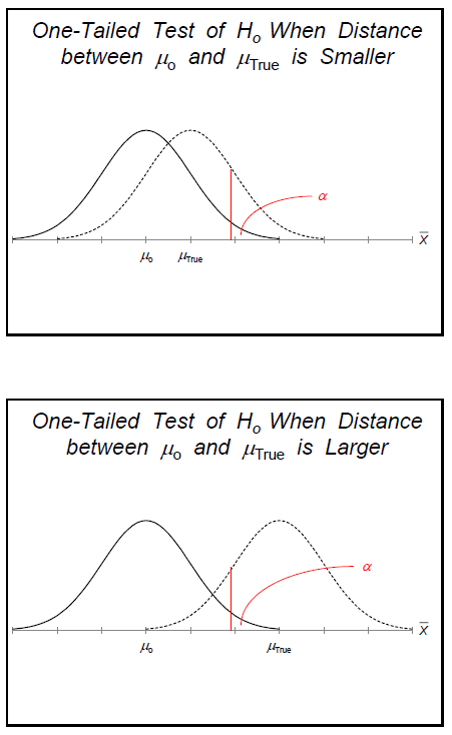
\includegraphics[width=3.5in]{prac_num.png}
\caption{}
\end{figure}

\section{Test Statistic Denominator}\label{test-statistic-denominator}

\begin{enumerate}
\def\labelenumi{\arabic{enumi}.}
\itemsep1pt\parskip0pt\parsep0pt
\item
  The standard error
\item
  This measures only random variation
\item
  Other things being equal, the larger the sample size, the smaller the
  standard error
\item
  If you have a very large sample size, the standard error can be very
  small.

  \begin{itemize}
  \itemsep1pt\parskip0pt\parsep0pt
  \item
    Therefore, even with a very small difference between observed mean
    and hypothesized mean, you can end up with a large value for the
    test statistic, thus leading to a statistically significant result.
  \end{itemize}
\item
  However, the result may not be of practical importance - too small to
  make a difference in the real world.
\end{enumerate}

\begin{figure}[H]
\centering
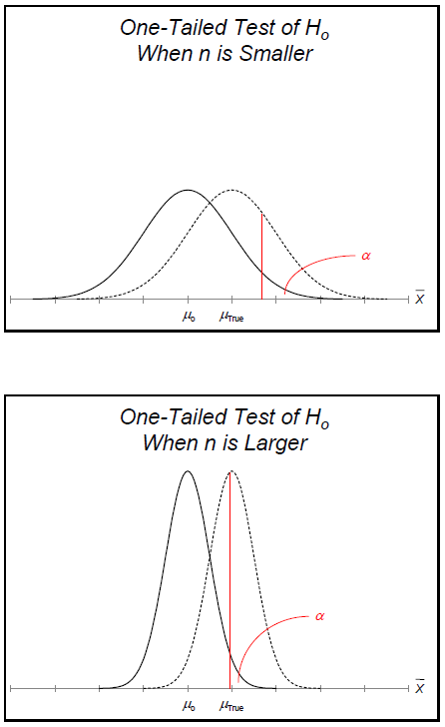
\includegraphics[width=3.5in]{prac_den.png}
\caption{}
\end{figure}

\section{Practical vs Statistical Significance
2}\label{practical-vs-statistical-significance-2}

\begin{itemize}
\itemsep1pt\parskip0pt\parsep0pt
\item
  In other words, with a large enough sample, even a very small
  difference between observed mean and hypothesized mean can lead to a
  rejection of the null hypothesis.
\item
  In cases like this, we have a result that is statistically
  significant, but in which the difference between hypothesized mean and
  true mean is so small as to be unimportant in a practical sense.
\end{itemize}

\section{Type I Errors, Type II Errors, and
Power}\label{type-i-errors-type-ii-errors-and-power}

\begin{itemize}
\itemsep1pt\parskip0pt\parsep0pt
\item
  \(Pr(\mbox{Reject true } H_{0}) = Pr(\mbox{Type I Error}) = \alpha\)
\item
  \(Pr(\mbox{Reject false } H_{0}) = Pr(\mbox{Type II Error}) = \beta\)
\item
  \(Pr(\mbox{Reject false } H_{0}) = Power = 1 - \beta\)
\item
  As \(\alpha\) increases (decreases)

  \begin{itemize}
  \itemsep1pt\parskip0pt\parsep0pt
  \item
    Power increases (decreases)
  \item
    \(\beta\) decreases (increases)
  \end{itemize}
\item
  Changing the sample size does not affect \(\alpha\)

  \begin{itemize}
  \itemsep1pt\parskip0pt\parsep0pt
  \item
    As n increases, \(\beta\) decreases, power increases, \(\alpha\)
    does not change.
  \end{itemize}
\end{itemize}

\section{Type I Errors, Type II Errors, and Power
Examples}\label{type-i-errors-type-ii-errors-and-power-examples}

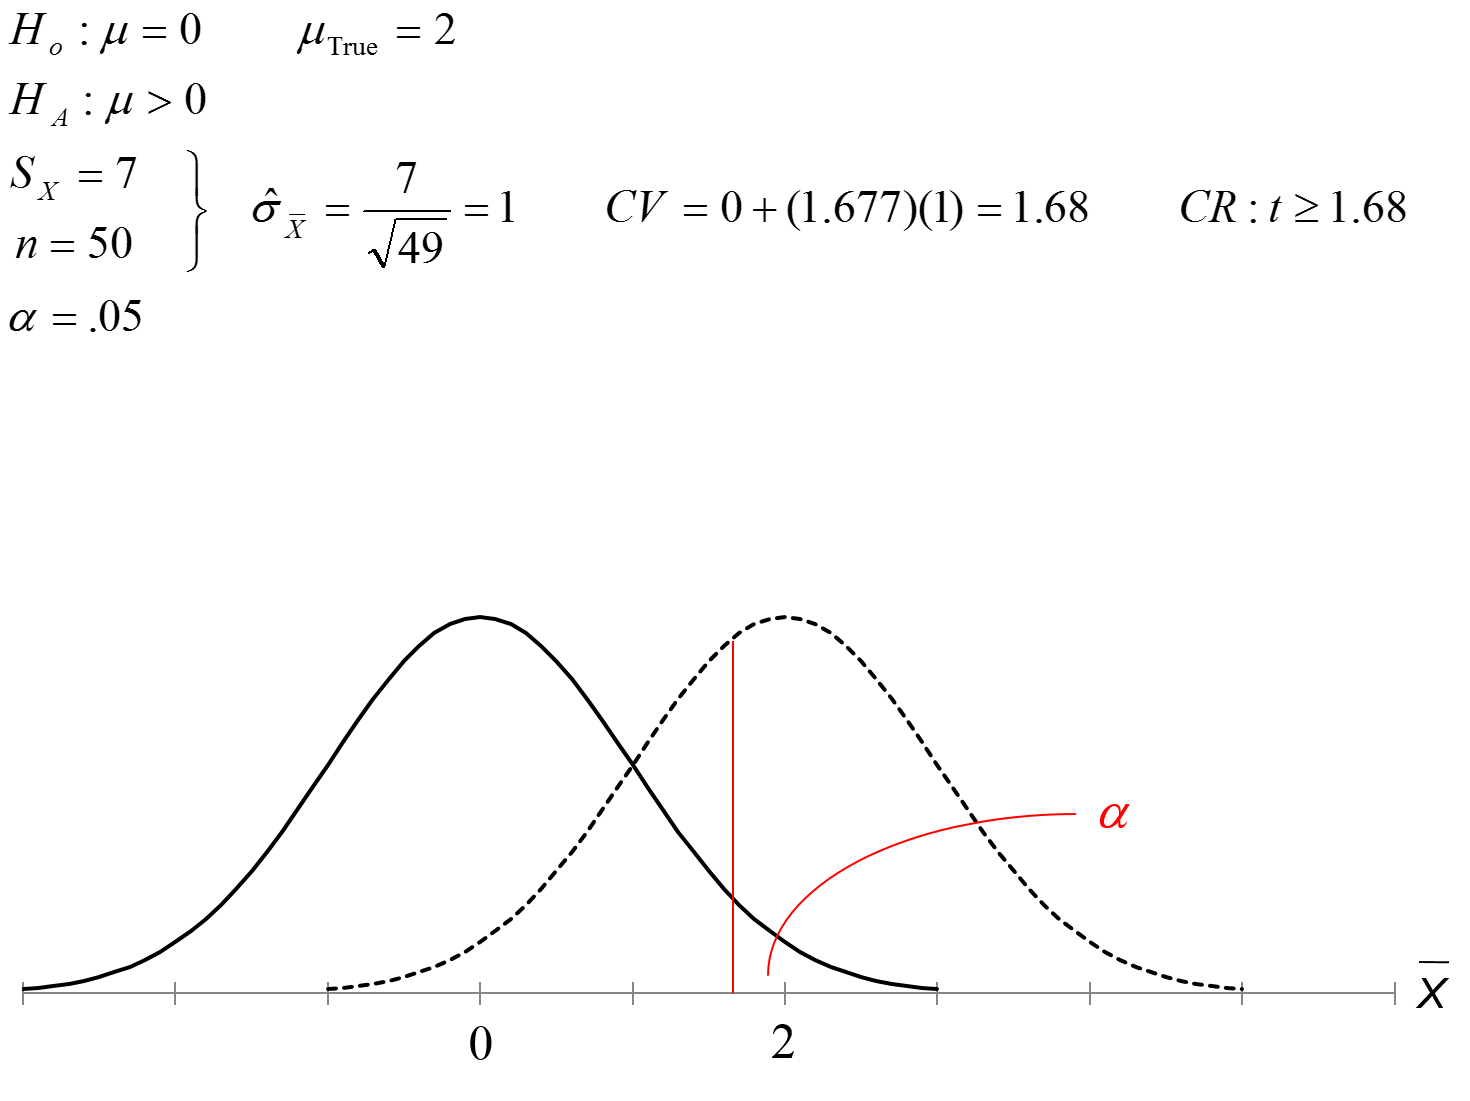
\includegraphics[width=3.5in]{t1e_examp.png} 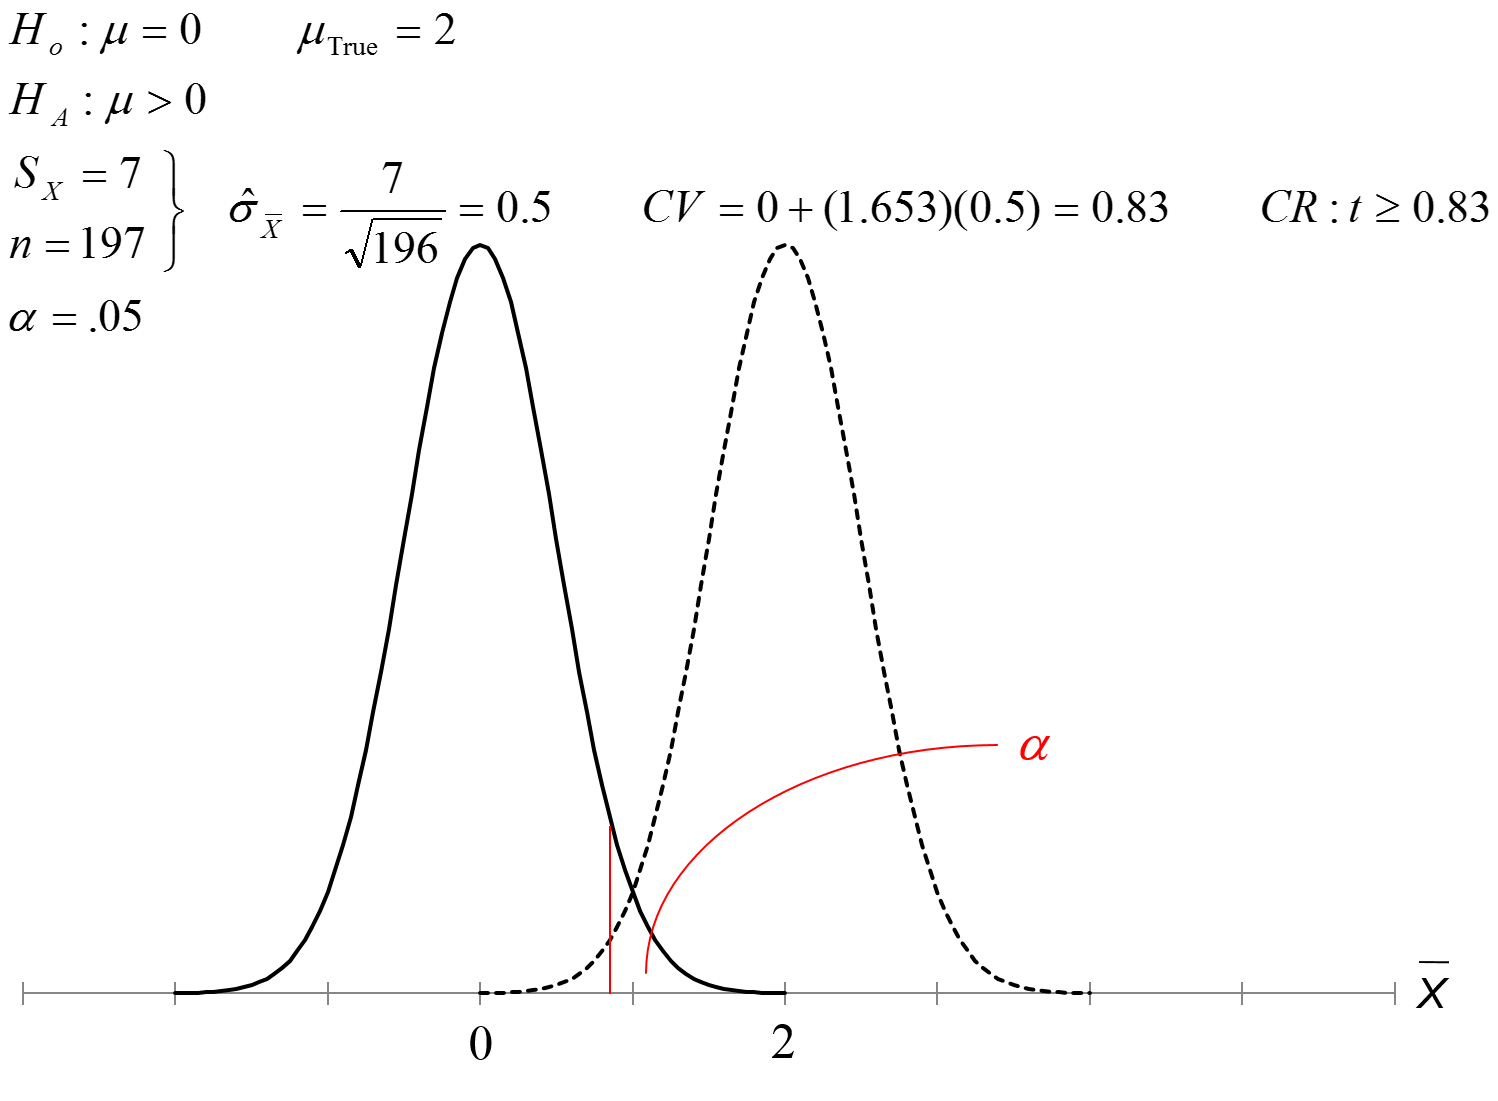
\includegraphics[width=3.5in]{t1e_examp2.png}

\section{\texorpdfstring{Calculating \(\beta\) and
Power}{Calculating \textbackslash{}beta and Power}}\label{calculating-beta-and-power}

\begin{figure}[H]
\centering
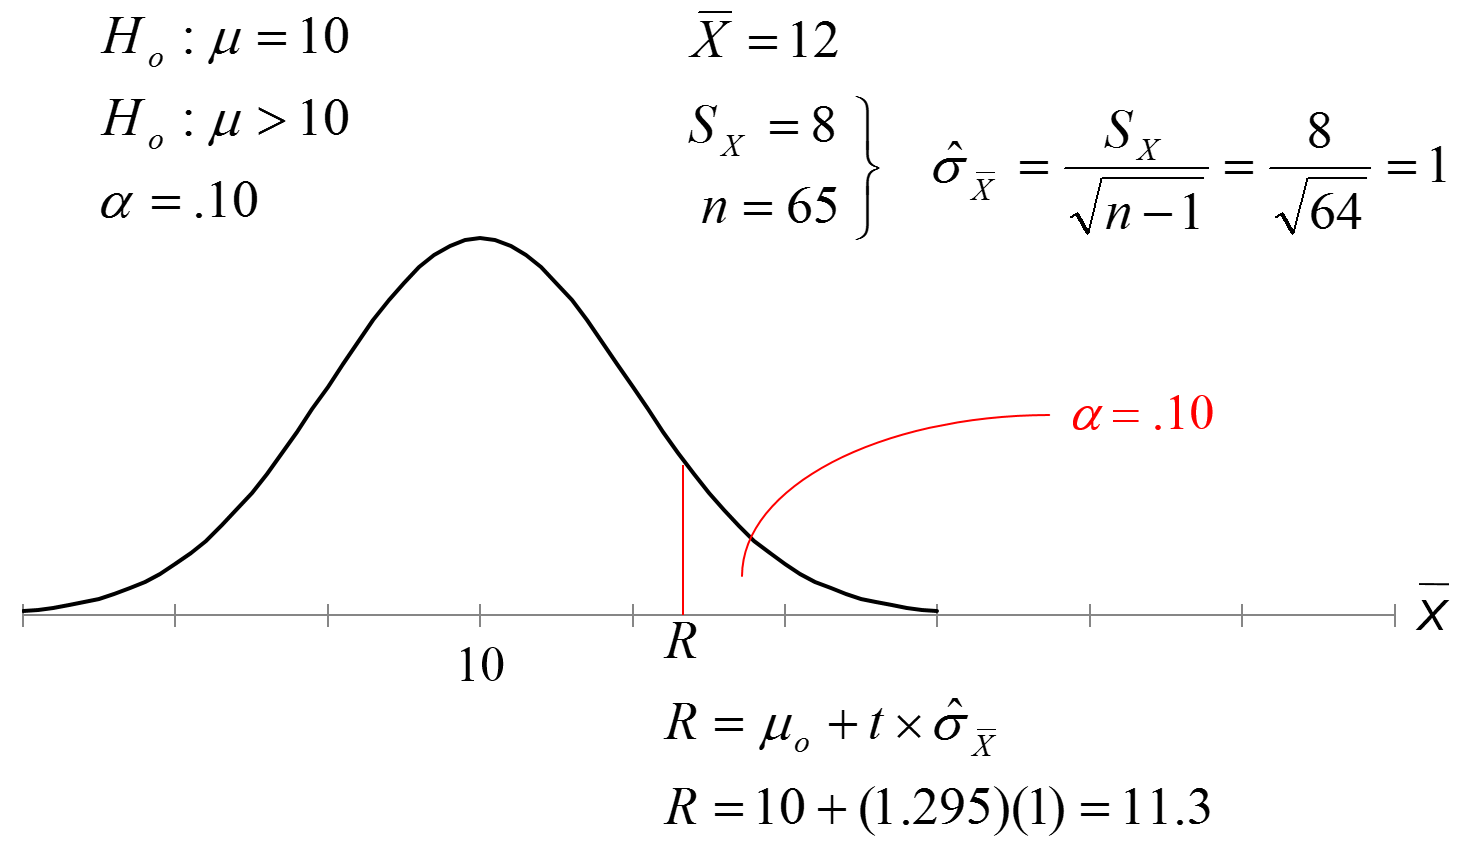
\includegraphics[width=3.5in]{Calc_power1.png}
\caption{}
\end{figure}

\begin{itemize}
\itemsep1pt\parskip0pt\parsep0pt
\item
  Suppose \(\mu_{true} = 12\) for this example.
\end{itemize}

\section{Power Curve}\label{power-curve}

\begin{figure}[H]
\centering
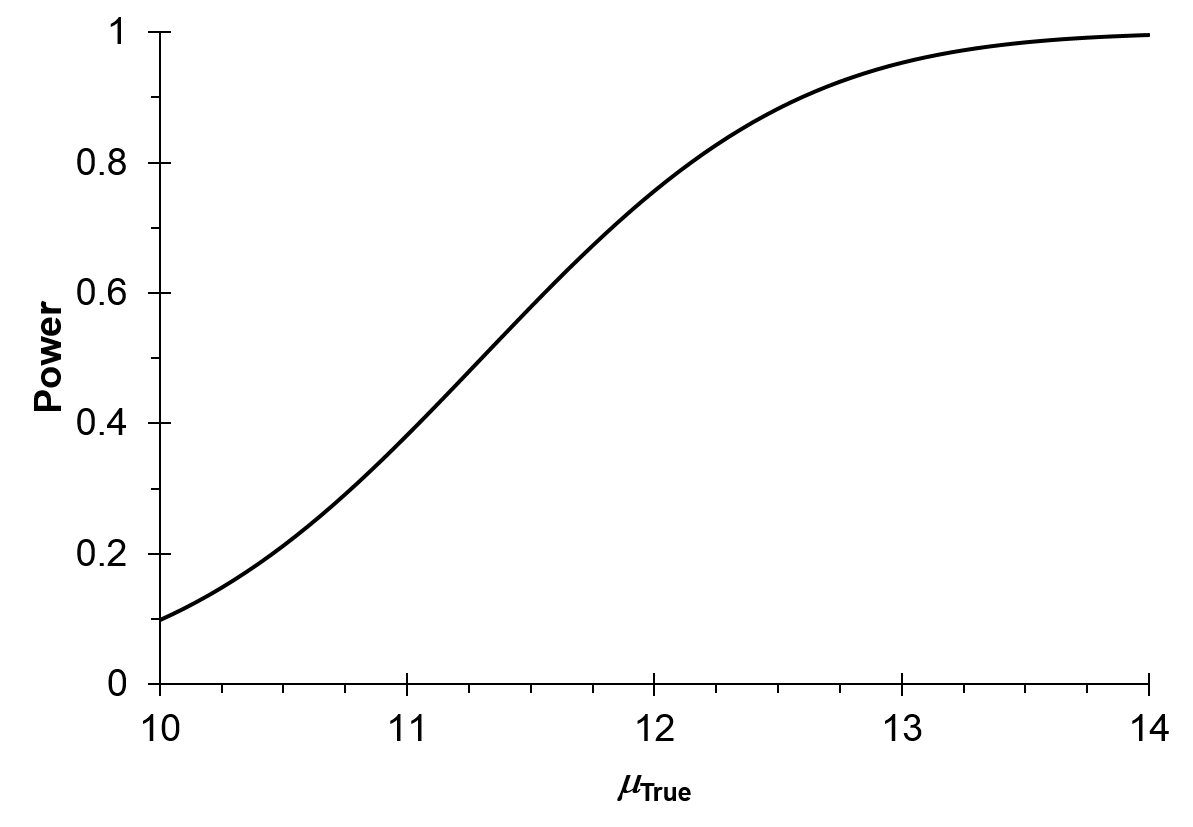
\includegraphics[width=3.5in]{power_curve.png}
\caption{}
\end{figure}

\end{document}
